% !TEX TS-program = pdflatex
% !TEX root = ../tesi.tex

\chapter{Cenni Storici}

\section {Inquinamento acustico e mare}
\begin{figure}[h]
\centering
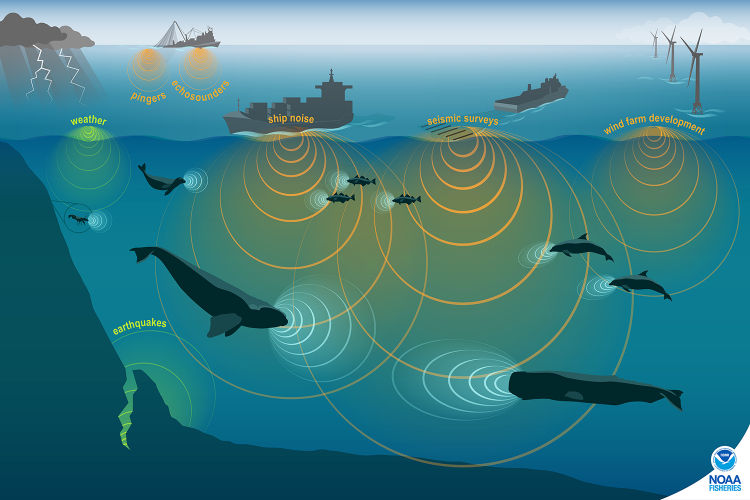
\includegraphics[width= .45\textwidth]{Worldrise_SeaMag_InquinamentoAcustico}
\caption{I suoni del mare: fonti sonore umane, animali e ambientali, con le rispettive onde sonore, approssimativamente proporzionali}
\end{figure}

Il suono è prodotto dalla vibrazione di un corpo che, oscillando, genera una variazione di pressione del mezzo in cui è immerso, provocando una serie di compressioni e rarefazioni che si propagano come onde sonore, fino a raggiungere l’apparato uditivo. 
Per propagarsi, il suono ha bisogno appunto di un mezzo, sia esso liquido, gassoso o solido, a seconda del quale varia la velocità e la propagazione dell’onda. 
Il suono viaggia nell’aria ad una velocità di circa 330 m/s e ancora più rapidamente nell’acqua, dove si sposta ad una velocità di circa 1500 m/s: l’acqua, infatti, essendo un mezzo meno comprimibile dell’aria permette di trasmettere la vibrazione più velocemente.

Le caratteristiche del mezzo, come per esempio la densità, che sott’acqua dipende da pressione, temperatura e salinità, modificano quindi la velocità di propagazione del suono.
In mare, il suono viaggia più velocemente nelle acque calde superficiali e più lentamente in quelle fredde e profonde. 
In profondità, inoltre, quando la pressione della colonna d’acqua sovrastante arriva a controbilanciare l’abbassamento di temperatura, la velocità ricomincia a crescere e nell’oceano più profondo il suono viaggia più rapidamente che in superficie. 
Nell’ambiente marino il suono può percorrere notevoli distanze, soprattutto quello a bassa frequenza, che può essere udito anche in aree molto vaste, fino al livello di interi bacini oceanici. Pertanto, i rumori generati sulla terraferma possono essere percepiti anche nelle profondità dell’oceano e ciò può avere un impatto significativo per la fauna marina.
Oltre che da bellissimi suoni, gli ambienti marini sono investiti anche dai rumori generati dalle attività antropiche. 
Le sorgenti principali di rumore sono: la navigazione, l’attività di estrazione di gas e petrolio dai fondali, la ricerca dei relativi giacimenti e l’utilizzo dei sonar attivi nelle navi. 
A queste si aggiunge anche l’attività di dragaggio, di costruzione delle strutture in mare e l’uso dei dispositivi pinger, che emettono suoni tali da allontanare i mammiferi marini e altre specie da attrezzature da pesca e impianti di acquacoltura.
Le navi sono tra le sorgenti più impattanti quando si parla di inquinamento acustico:  basti pensare che solamente il suono prodotto dalla cavitazione dell’elica, quando intorno all’elica viene a formarsi un vuoto d’acqua, può diffondersi in un raggio di centinaia di chilometri intorno alla nave che lo ha generato. 
Il rumore della navigazione cambia inoltre a seconda della tipologia, dimensione e velocità dell’imbarcazione.
Anche la ricerca dei giacimenti di combustibili fossili è particolarmente impattante dal punto di vista acustico e sempre più frequentemente viene impiegato il sistema delle prospezioni sismiche, ecologicamente molto distruttivo. 
Il metodo consiste infatti nella scansione della zona prescelta mediante dei dispositivi che, trainati da navi, emettono suoni ad altissimi livelli di pressione e la cui eco, riflessa dal fondale, rivela presenza, profondità e tipologia del giacimento.

\begin{figure}[h]
\centering
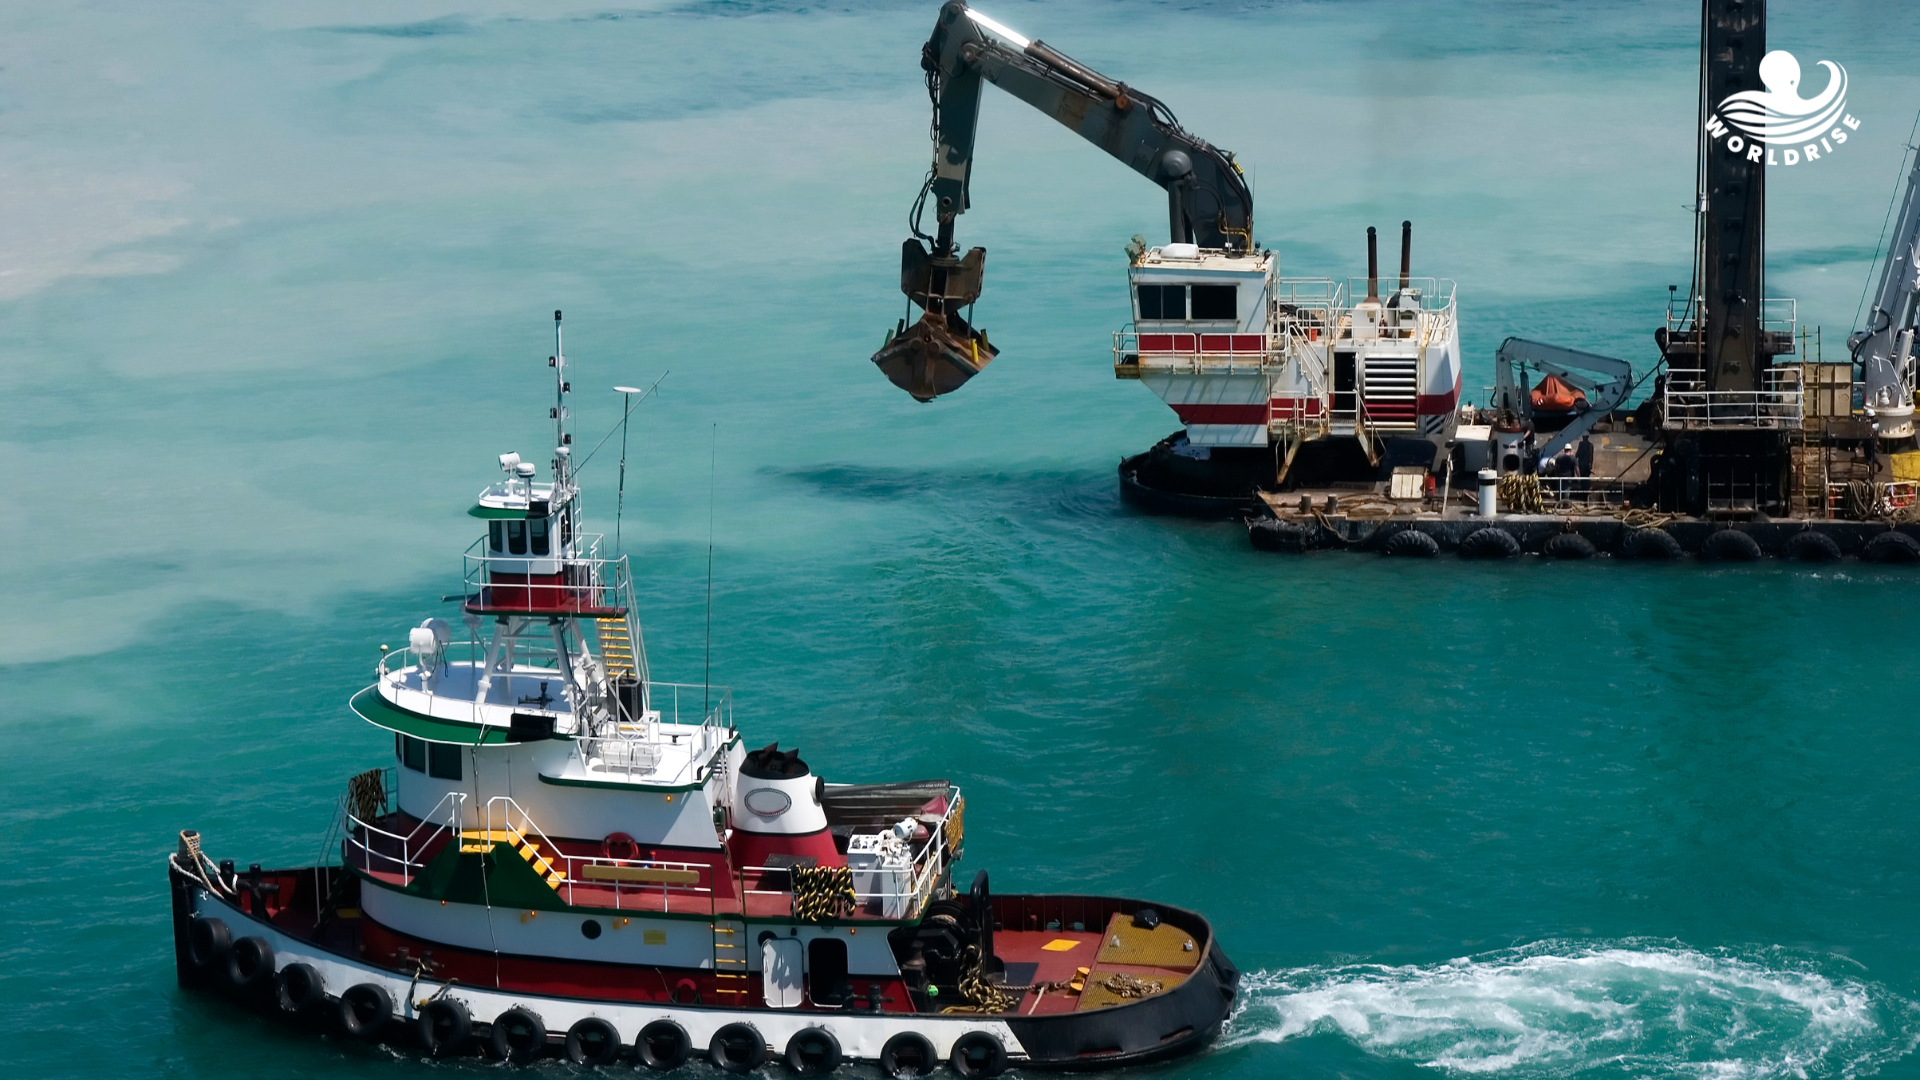
\includegraphics[width= .45\textwidth]{dragaggio}
\caption{Dragaggio}
\end{figure} 

L’inquinamento acustico marino è oggetto di studio solo da poco tempo, ma negli ultimi anni sono sempre più documentati gli impatti per la fauna marina. 
In particolare, è stato provato il danno causato a molte specie dal rumore dei sonar delle imbarcazioni, le cui onde sonore si possono diffondere per centinaia di chilometri in mare, provocando negli animali anomalie nel comportamento, perdita dell’udito, lesioni gravi e anche la morte. 
Infatti, numerosi sono gli spiaggiamenti di mammiferi marini rinvenuti durante le esercitazioni di navi militari che utilizzavano i sonar.

Un ulteriore rumore pericoloso per la fauna marina è quello causato dalle navi mercantili, che viene emesso ad una frequenza tale da interferire con i suoni prodotti dagli animali, soprattutto delle balene. 
Molti animali, a causa dell’inquinamento acustico, hanno cambiato le proprie abitudini: nell’Artico, per esempio, alcuni hanno deviato le proprie rotte di migrazione, come il beluga che cerca di evitare le imbarcazioni che navigano nei mari artici. 
Inoltre, è stato segnalato dall’ IPCC (Panel Intergovernativo sui Cambiamenti Climatici) che l’acidificazione dei mari, causata da un incremento di CO2 disciolta in acqua, può accrescere l’inquinamento acustico sottomarino, poiché diminuisce la capacità dell’acqua di assorbire i suoni a bassa frequenza.
I rumori delle attività antropiche disturbano gli abitanti del mondo sottomarino, tanto che si parla di “inquinamento acustico”. 
Nella Convenzione sul diritto del mare del 1982 questo fenomeno è definito come “l’introduzione diretta o indiretta, conseguente alle attività umane, di sostanze o energia nell’ambiente marino, compreso il rumore sottomarino prodotto dall’uomo, che provoca o che può provocare effetti deleteri come danni alle risorse biologiche e agli ecosistemi marini, inclusa la perdita di biodiversità”. 
È un problema ambientale che deve essere affrontato per tutelare l’ecosistema marino, agendo sulle fonti che generano i rumori impattanti.

L’Unione Europea, per prima a livello globale, ha adottato a fine novembre 2022 una raccomandazione sui livelli massimi accettabili di rumore sottomarino, nel quadro del Zero Pollution Action Plan. 
Si distinguono due forme di rumore, quello continuo, come il traffico marittimo, che incide per il 27\% dell’area marina europea, e quello impulsivo o temporaneo, come l’estrazione di gas e petrolio. 
È stabilito che, per proteggere l’ambiente sottomarino:
\begin{itemize}
\item non più del 20\% di un’area può essere esposta a rumori continui in un anno;
\item non più del 20\% dell’area può essere esposta a rumori temporanei in un giorno;
\item non più del 10\% dell’area può essere esposta a rumori temporanei in un anno.
\end{itemize}

Tali soglie sono state sviluppate all’interno della Marine Strategy Framework Directive, che ha come obiettivo quello di monitorare, valutare e implementare misure per proteggere l’ecosistema marino. 
Ogni Stato Membro dovrà quindi sviluppare delle proprie strategie per rispettare tali limiti. 
Inoltre, la riduzione del rumore prodotto dalle navi è un tema su cui anche l’International Maritime Organisation (IMO), l’istituto delle Nazioni Unite che si occupa di rendere il trasporto marittimo internazionale più sicuro e sostenibile, sta ponendo attenzione.

\begin{figure}[h]
\centering
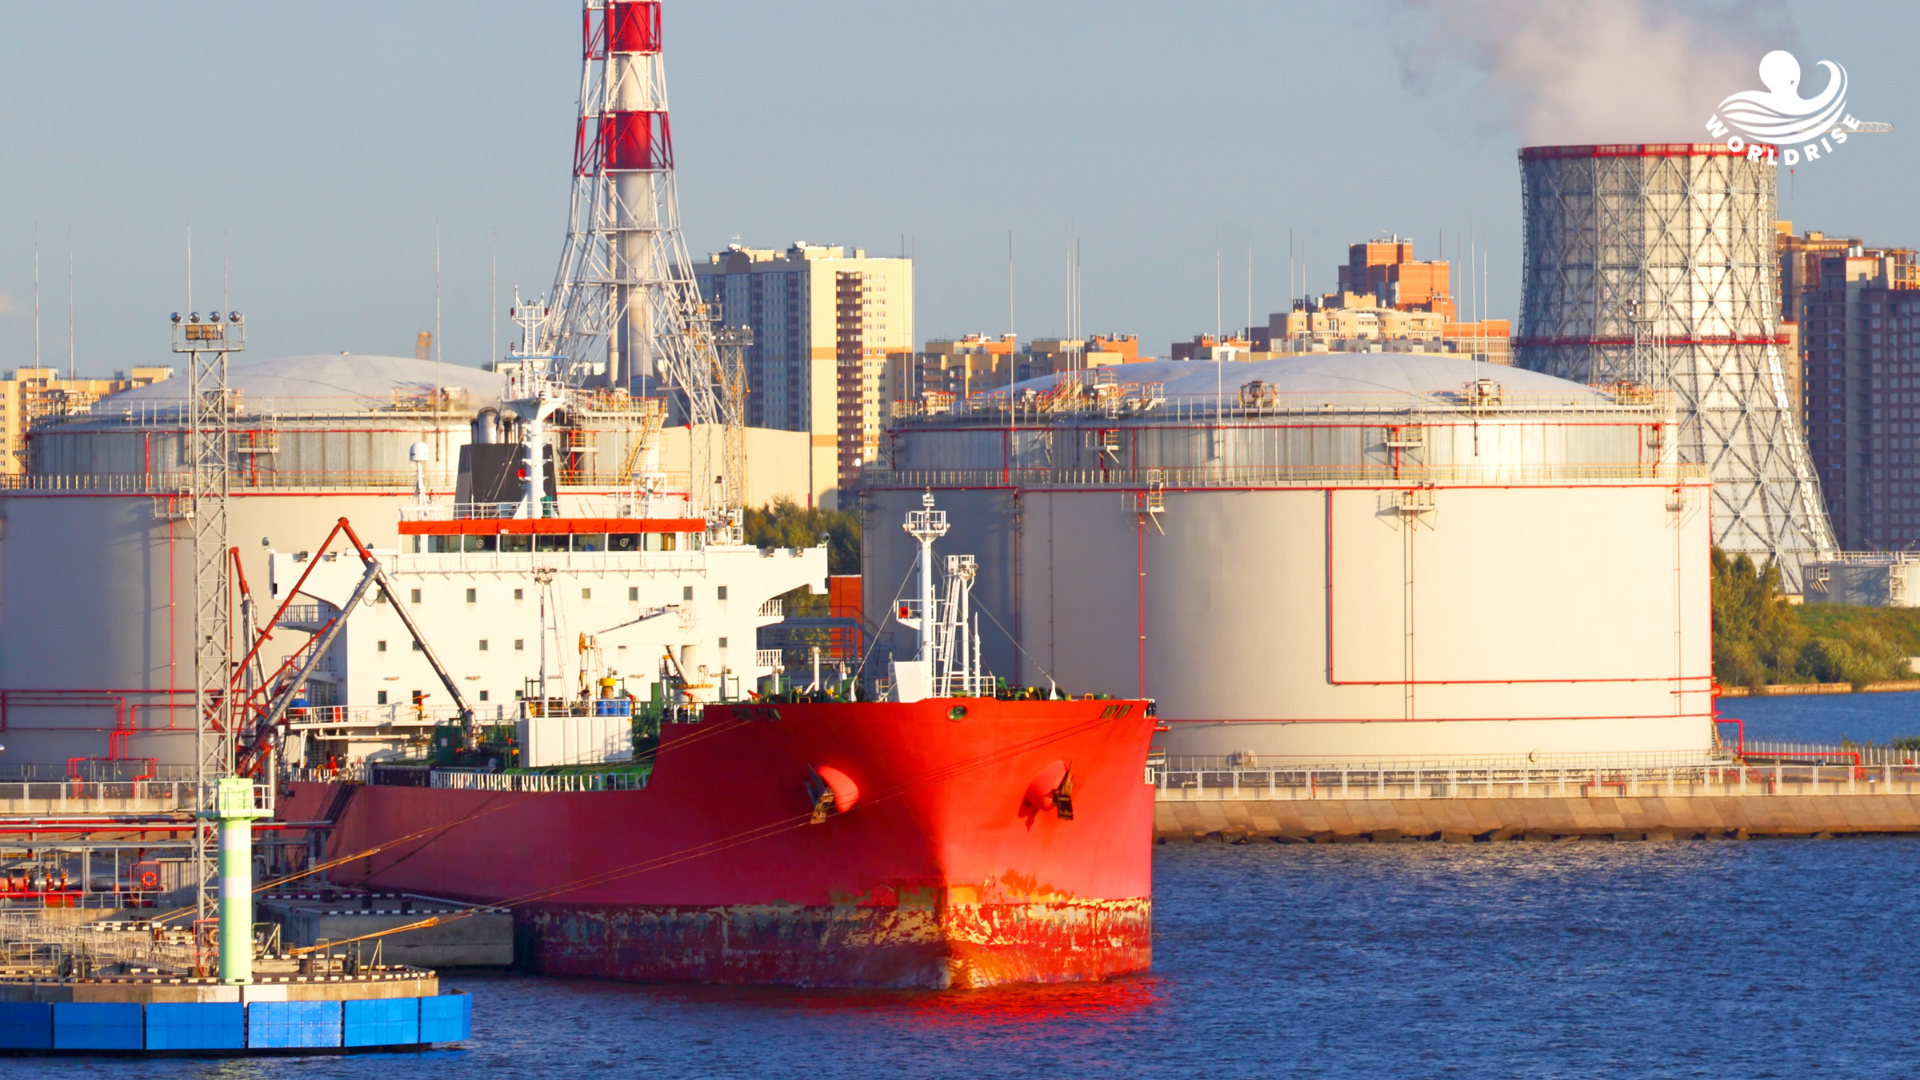
\includegraphics[width= .45\textwidth]{Worldrise_SeaMag_InquinamentoAcustico-6}
\caption{Porto Marittimo}
\end{figure}

\section{L'idrofono}

Un idrofono è uno strumento elettroacustico per rivelare suoni in un liquido (generalmente acqua) e determinare la direzione della loro sorgente. 
Il principio di funzionamento è simile a quello del microfono che in aria trasforma le vibrazioni di una sottile membrana dovute al transito dell’onda acustica, in segnali elettrici elaborabili. 
In acqua la membrana è sostituita da un diverso trasduttore. 
Negli idrofoni comuni si utilizzano sensori piezoelettrici nei quali la pressione dell’onda acustica sulle superfici di un opportuno materiale cristallino genera un segnale elettrico.

Questo strumento è largamente utilizzato in marineria per rivelare la presenza di navi tramite la ricezione dei rumori subacquei generati dall'elica in movimento e dai motori. 
Gli idrofoni furono sviluppati in modo intensivo durante la guerra 1914-18 per consentire ai cacciasommergibili di scoprire la presenza di sommergibili nemici immersi. 
Lo sviluppo dell’idrofono avvenne contemporaneamente in vari paesi, dunque non ne esiste un unico, definito inventore. 

Vanno ricordati: L. Nixon che per primo cercò di rivelare la presenza di iceberg con un rivelatore passivo di suoni (1906), A Blem in Vienna (1912), Lewis Richardson in Gran Bretagna (1913 primo brevetto eco-scandaglio), il canadese Reginald Fessenden negli Stati Uniti (1914 primo SONAR), Il fisico francese Paul Langévin e Constantin Chilowsky ingegnere russo immigrato in Francia (brevetto di un SONAR che battezzarono hydrophone 1915) e, infine, il fisico canadese R.W. Boyle , studioso di ultrasuoni e delle loro applicazioni alla University of Alberta, che dal 1916 brevettò un SONAR poi ulteriormente sviluppato dallo stesso R.W. Boyle nei laboratori della Royal Navy. 
Nel 1918 il gruppo di Boyle sviluppò un SONAR capace di individuare la presenza di sommergibili ad una distanza di 1800 metri che venne installato negli anni successivi sulle unità della marina inglese.

Questo strumento si è diffuso moltissimo, non solo per i possibili usi militari, ma anche negli studi oceanografici, nelle ricerche biologia marina, nella protezione dei parchi marini, nella prevenzione dai terremoti e dagli tsunami, e in tutta la marineria commerciale e turistica. L’idrofono è infatti l’unità ricevente di ogni eco-scandaglio, uno strumento di grande uso, presente ormai in ogni imbarcazione di diporto per identificare gli scogli sommersi, la presenza di branchi di pesci o la profondità della scogliera.

Nell’acque marine in superficie e ad una temperatura di 20 °C il suono si trasmette ad una velocità di circa 1521 metri al secondo cioè 4,5 volte superiore a quella nell'aria. 
L’assorbimento del suono in acqua è invece molto minore. 
Oggi gli idrofoni, anche grazie allo sviluppo delle moderne tecniche di trasformazione dell’onda sonora in segnale elettronico o opto-elettronico, consentono quindi di captare anche suoni emessi a grandi distanze. 
La direzione della sorgente viene determinata dallo sfasamento dell’onda sonora tra idrofoni posti a vari metri di distanza.

Più complesso è determinare la distanza della sorgente.
 Il metodo utilizzato è quello di misurare il tempo che impiega un’onda sonora a raggiungere il corpo da monitorare e a ritornare riflessa alla sorgente. 
In questo caso si può scoprire la presenza e determinare la distanza di un oggetto in acqua anche se esso non produce onde sonore: è quanto avviene negli eco-scandagli o nei sonar. 
L’idrofono è l’unità ricevente anche di molti altri strumenti usati in ingegneria idraulica come, ad esempio, misuratori di portata, di pressione in condutture idrauliche o di sensori per la rilevazione di correnti in profondità in bacini marini o lacustri.

Gli idrofoni sono largamente diffusi nelle ricerche di biologia marina per conoscere abitudini e tracciare le migrazioni dei grandi cetacei, delle balene o dei delfini senza introdurre perturbazioni o presenze inadatte al loro habitat naturale, o anche per studiare l’utilizzo della comunicazione sonora dei mammiferi marini. 
Sono anche utilizzati per misurare temperatura, salinità e pressione (direttamente correlata con la profondità) locali. 
La velocità dell’onda acustica varia infatti con le proprietà dell’acqua. 

Ad esempio: un aumento di 1°C grado Celsius dell’acqua marina determina un aumento della velocità dell’onda acustica di 4 metri al secondo, la variazione di pressione dovuta a un chilometro di inabissamento provoca una crescita della velocità di 1,4 metri al secondo. 
Le variazioni globali del clima sono controllabili tramite la tomografia acustica di vaste zone degli oceani (milioni di chilometri quadrati). Idrofoni sono anche utilizzati per la protezione da terremoti terrestri. 

L’idrofono ha una sua ampia utilizzazione nei modem acustici per la trasmissioni dati attraverso l’acqua. 
Le onde radio non si trasmettono sottacqua, i sistemi di trasmissione dati sommersi sono quindi basati sulla trasmissione cablata (fibre ottiche) o su quella sonora. 
Nei modem acustici si tratta di trasformare un segnale digitale in onde sonore, e poi di riconvertirlo. 
Come accade con la tradizionale “modulazione” sulle linee telefoniche analogiche (quella che usa uno strumento chiamato modem, cioè un modulatore e de-modulatore). 
I modem acustici, quantunque la velocità di trasmissione sia molto inferiore a quella dell’onda elettromagnetica in aria (onde radio) o su cavo, realizzano attualmente una ottima soluzione alla trasmissione dati wireless in acqua tra stazioni sommerse (subsea) e dall’acqua da stazioni sommerse ad una centrale emersa (topsea). 
Questi nuovi sistemi sono di grande utilità nell’oceanografia e in molte altre applicazioni scientifiche, civili e militari e sono quindi in grande, rapida, espansione. 

Idrofoni di particolare sensibilità sia con le tradizionali tecniche pizio-elettriche , sia con innovative tecniche FBG utilizzano fibre ottiche con reticoli di Bragg (FBG) , sono oggi proposti per essere utilizzati in ricerche di fisica sub-nucleare o astrofisica per rilevare il passaggio di particelle in un mezzo liquido.

\section {Sonar e la sua nascita}

Venne inventato da Paul Langevin nel 1917. 
La marina inglese e quella tedesca considerarono il sottomarino, nel periodo tra le due guerre, un'arma superata soprattutto dopo l'avvento del dispositivo di rilevazione acustica detto "ASDIC" (Anti-Submarine Detection Investigation Committee), noto oggi come sonar; furono i britannici i primi a sviluppare una tecnologia che permettesse di rilevare un oggetto attraverso il suono, e la scoperta del propagarsi delle onde sonore in acqua non era avvenuta durante la prima guerra mondiale e, per il rilevamento dei sommergibili, erano utilizzati dei semplici idrofoni). 
Il sistema ASDIC era composto da un trasduttore, contenuto in una cupola sotto la nave, che inviava onde acustiche che tornavano all'origine se riflesse da un oggetto sommerso, posto ad una distanza massima di circa 2700 m. 
La cupola poteva essere fissa, come nell'apparato Type 123 installato sulle corvette della classe Flower o retrattile come in alcune navi, quali il cacciatorpediniere HMS Campbeltown, dotato di un ASDIC Type 124. 
Dall'eco veniva ricavata la direzione e la distanza dell'oggetto ma falsi segnali potevano essere generati dalle differenze di temperatura dell'acqua, correnti, banchi di pesci (strato riflettente profondo), ed inoltre l'ASDIC era efficace solo a velocità inferiori ai 15 nodi (28 km/h), poiché a velocità superiori il rumore della nave avrebbe coperto gli echi; un ulteriore limite era rappresentato dal brandeggio del trasduttore, solo in senso orizzontale, con la conseguenza che il contatto veniva perso quando il bersaglio passava sotto la nave cacciatrice.

La procedura di utilizzo consisteva nell'uso dell'ASDIC in un arco da un lato all'altro della nave, fermando il trasduttore a distanze di pochi gradi per inviare un segnale, e le ricerche in gruppi di navi prevedevano l'allineamento delle navi a distanza compresa tra il miglio ed il miglio e mezzo; se veniva captata un'eco identificabile come sottomarino la nave avrebbe puntato verso il bersaglio e si sarebbe avvicinata a media velocità fino a trovarsi ad una distanza inferiore alle 1000 yard (910 m) e, nel frattempo, tramite il plotter veniva tracciata la direzione e la distanza, in modo da ricavare la rotta del sottomarino e la sua velocità. 
L'attacco veniva portato passando davanti al sottomarino per scaricare le bombe di profondità, lanciandole ad intervalli, seguendo uno schema tale da intrappolare il sottomarino. 
Per essere efficaci tuttavia, le bombe dovevano esplodere ad una distanza inferiore ai 6 metri e i primi sistemi ASDIC non erano in grado di determinare la profondità con sufficiente precisione; per questo motivo lo schema di sganciamento delle bombe prevedeva anche l'esplosione delle stesse a diverse profondità.

Il sistema ASDIC soffriva di alcuni limiti:
\begin{itemize}
\item gli U-Boot potevano scendere a profondità maggiori rispetto a quelli britannici e statunitensi, pari a 210 m, oltre le capacità delle bombe di profondità britanniche, che potevano raggiungere circa 100 m, e l'esplosione di una bomba di profondità disturbava l'acqua, rendendo molto difficile la riacquisizione del contatto nemico se falliva il primo attacco; è da rilevare inoltre che il sistema non godeva della fiducia delle marine alleate e la Royal Navy iniziò la guerra con un numero insufficiente di cacciatorpediniere e di ufficiali esperti in armi antisommergibile. La situazione nel comando costiero della Royal Air Force era ancora più grave, poiché gli aerei da ricognizione non possedevano adeguata autonomia per il pattugliamento e non erano ancora state valutate le conseguenze che la scoperta del radar avrebbe avuto nella guerra sul mare.
\end{itemize}

Anche altre marine iniziarono a sperimentare i primi modelli di ASDIC quando alcune unità, corvette ma anche pescherecci armati, vennero equipaggiati con personale non inglese, o apparati vennero installati su navi alleate, come il cacciatorpediniere olandese Isaac Sweers.

In Italia lo studio e la costruzione dei sonar riprende dopo la seconda guerra mondiale nel 1951.

I primi sonar italiani per sottomarini, costruiti tra il 1960 e 1974, erano identificati con le sigle: IP60 - IP64 e IP70 - IP74S. 
Il loro nome, coniato in Italia, era: Apparati Ecoidrofonici.

\begin{figure}[h]
\centering 
\subfloat [Sottomarino CI. Toti (1967)]
{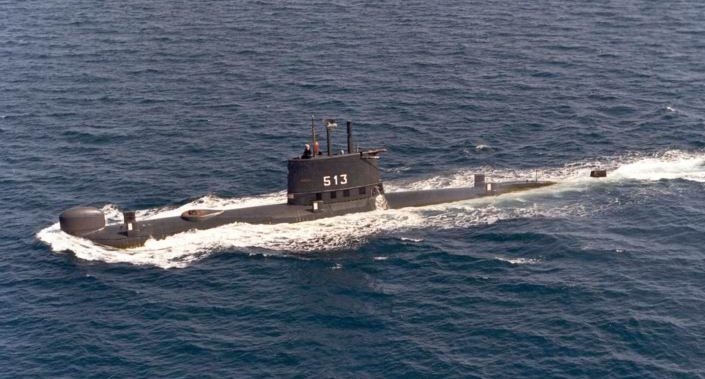
\includegraphics[width=.45\columnwidth]{SOTTOMARINO CI 1967}} \quad
\subfloat [Sottomarino CI Sauro (1976)]
{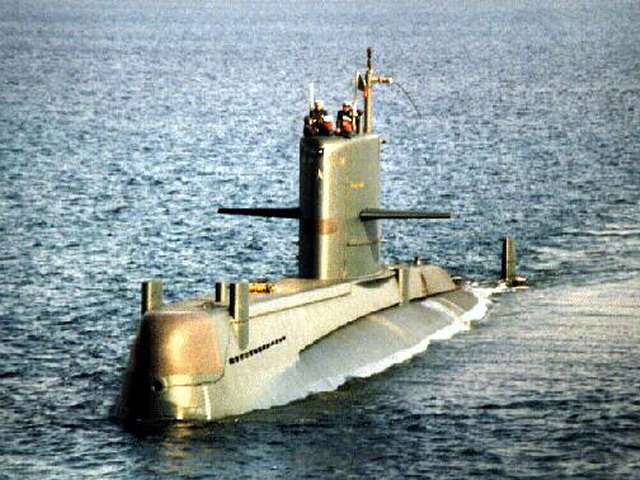
\includegraphics[width=.45\columnwidth]{SOTTOMARINO CI SAURO}} \quad
\subfloat[Sottomarino CI U212 (2003)]
{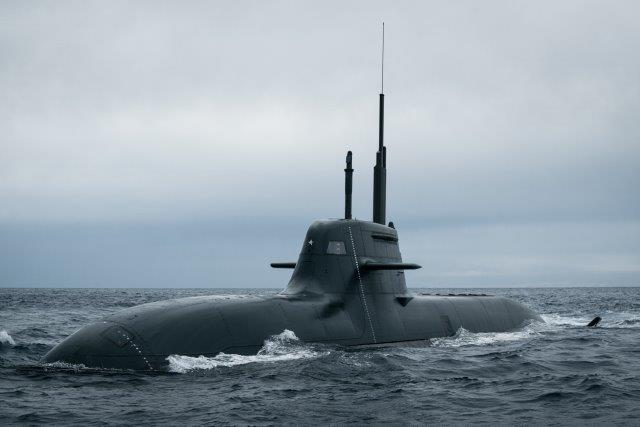
\includegraphics[width=.45\columnwidth]{SOTTOMARINO CI}} \quad
\caption [Sottomarini in italia dal 1960 ad oggi]{Sottomarini in Italia dal 1960 ad oggi}
\end{figure}

